%!TEX root = ../../thesis.tex
\chapter{Parametric Inference using Persistence Diagrams}
\label{ch:parametric_inference}

\epigraph{``I predict a new subject of statistical topology. Rather than count the
number of holes, Betti numbers, etc., one will be more interested in the
distribution of such objects on noncompact manifolds as one goes out
to infinity''}{Isadore Singer}

\section{Introduction}

Recent work in topological data analysis has concentrated on developing the statistical foundations for data analysis using the persistent homology framework (see the discussion in Section~\ref{bg:tda:ph:statistics} and references \cite{Fasy:2014,Blumberg:2014bq,Chazal:2014vl}).
The focus of this work has primarily been estimating the topology of an object from a finite, noisy sample.
Doing so requires statistical methods to distinguish topological signal from noise.

Here we consider a different scenario.
Many simple stochastic models generate complex data that cannot be readily visualized as a manifold or summarized by a small number of topological features.
The persistence diagrams generated from such models will be unique in two ways: (1) the complexity of the diagram (i.e. number of topological features) will grow with the number of sampled points, and (2) each instantiation of the model will generate a unique set of topological features.
Nevertheless, the collection of measured topological features may exhibit additional structure, providing useful information about the underlying data generating process.
While the persistence diagram is itself a summary of the topological information contained in a sampled point cloud, to perform inference further summarization may be appropriate, e.g. by considering distributions of properties defined on the diagram.
In other words, we are less interested in learning the topology of a particular sample, but rather in understanding the expected topological signal of different model parameters.
We show an example in Figure~\ref{fig:sim_barcodes}.
Here we have three identical simulations of a stochastic coalescent model, commonly used in population genetics.
Each simulation is generated with the same number of points and the same parameters.
Because the model is random, the resulting topology will also be random, making it impossible to match individual topological features between diagrams.
We would like a way to characterize these models using topology.

In this chapter, we show that summary statistics computed on the persistence diagram can be used for likelihood-based parametric inference.
We use genomic sequence data as a case study, examining the topological behavior of the coalescent process with recombination, a widely used stochastic model of biological evolution.
We find that the process generates nontrivial topology in a way that depends sensitively on parameters in the model.
The idea is presented as a proof of concept, in order to motivate the identification additional models with regular topological structure that may amenable to this type of inference.

\begin{figure}
\centering
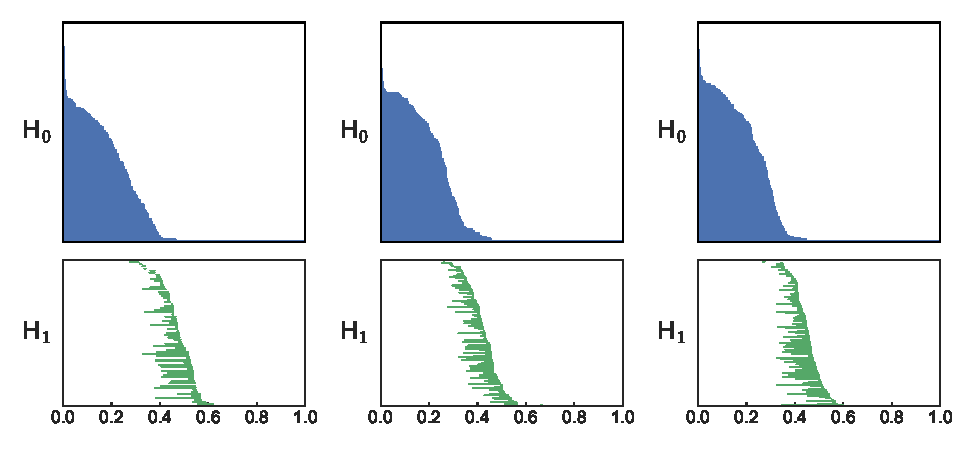
\includegraphics[width=\textwidth]{fig/parametric_inference/sim_barcodes.pdf}
\caption[Barcode Diagrams for Three Coalescent Simulations]{Barcode diagrams for three simulations of a stochastic coalescent model. Each simulation is generated using the same parameters, however as random models the persistent homology will differ for each run. Simulations were performed in \texttt{ms} using the command \texttt{ms 200 1 -t 500 -r 144 10000}.}
\label{fig:sim_barcodes}
\end{figure}

% \section{Warmup: Gaussian Random Fields}

% Here we show that parametric inference of Gaussian Random Fields can be performed from the barcode diagram.
% Make reference to \cite{Adler:2010}.
% Connections with problems in cosmology.
% \kje{}

\section{The Coalescent Process}

The coalescent process is a stochastic model that generates the genealogy of individuals sampled from an evolving population \cite{Wakeley:2009}.
The genealogy is then used to simulate the genetic sequences of the sample.
This model is essential to many methods commonly used in population genetics.
Starting with a present-day sample of $n$ individuals, each individual's lineage is traced backward in time, towards a mutual common ancestor.
Two separate lineages collapse via a coalescence event, representing the sharing of an ancestor by the two lineages.
The stochastic process ends when all lineages of all sampled individuals collapse into a single common ancestor.
In this process, if the total (diploid) population size $N$ is sufficiently large, then the expected time before a coalescence event, in units of $2N$ generations, is approximately exponentially distributed:
\begin{equation}
P(T_{k}=t) \approx \binom{k}{2} e ^{-\binom{k}{2} t},
\end{equation}
where $T_k$ is the time that it takes for $k$ individual lineages to collapse into $k-1$ lineages.

After generating a genealogy, the genetic sequences of the sample can be simulated by placing mutations on the individual branches of the lineage.
The number of mutations on each branch is Poisson-distributed with mean $\theta t / 2$, where $t$ is the branch length and $\theta$ is the population-scaled mutation rate.
In this model, the average \emph{genetic distance} between any two sampled individuals, defined by the number of mutations separating them, is $\theta$.

The coalescent with recombination is an extension of this model that allows different genetic loci to have different genealogies.
Looking backward in time, recombination is modeled as a splitting event, occurring at a rate determined by population-scaled recombination rate $\rho$, such that an individual has a different ancestor at different loci.
Evolutionary histories are no longer represented by a tree, but rather by an \emph{ancestral recombination graph}.
Recombination is the component of the model generating nontrivial topology by introducing deviations from a contractibile tree structure, and is the component which we would like to quantify.
Coalescent simulations were performed using \texttt{ms} \cite{Hudson:2002}.

\begin{figure}
\begin{center}
\centerline{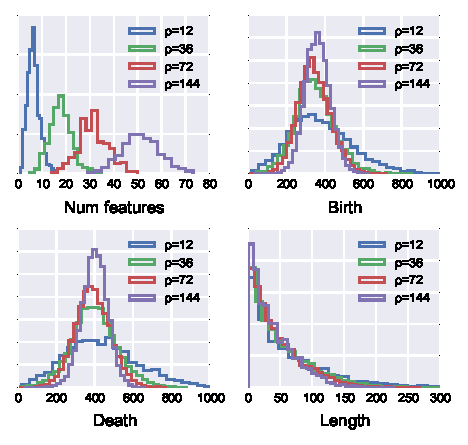
\includegraphics[width=\columnwidth]{./fig/parametric_inference/coalescent_sims.pdf}}
\caption[Distributions of statistics defined on the $H_1$ persistence diagram for different model parameters]{Distributions of statistics defined on the $H_1$ persistence diagram for different model parameters. Top left: Number of features. Top right: Birth time distribution. Bottom left: Death time distribution. Bottom right: Feature length distribution. Data generated from $1000$ coalescent simulations with $n=100$, $\theta=500$, and variable $\rho$.}
\label{fig:coalescent_sims}
\end{center}
\end{figure}

\section{Statistical Model}
\label{sec:model}

The persistence diagram from a typical coalescent simulation is shown in Figure \ref{fig:sim_barcodes}.
Examining the diagram, it would be difficult to classify the observed features into signal and noise.
Instead, we use the information in the diagram to construct a statistical model in order to infer the parameters, $\theta$ and $\rho$, which generated the data.
Note that we consider inference using only $H_1$ invariants, but the ideas easily generalize to higher dimensions.
We consider the following properties of the persistence diagram: the total number of features, $K$; the set of birth times, $(b_1,{\ldots},b_K)$; the set of death times, $(d_1,{\ldots},d_K)$; and the set of persistence lengths, $(l_1,{\ldots},l_K)$.
In Figure \ref{fig:coalescent_sims} we show the distributions of these properties for four values of $\rho$, keeping fixed $n=100$ and $\theta=500$.
Several observations are immediately apparent.
First, the topological signal is remarkably stable.
Second, higher $\rho$ increases the number of features, consistent with the intuition that recombination generates nontrivial topology in the model.
Third, the mean values of the birth and death time distributions are only weakly dependent on $\rho$ and are slightly smaller than $\theta$, suggesting that $\theta$ defines a natural scale in the topological space.
However, higher $\rho$ tightens the variance of the distributions.
Finally, persistence lengths are independent of $\rho$.

Examining Figure \ref{fig:coalescent_sims}, we can postulate: $K \sim \mathrm{Pois}(\zeta)$, $b_k \sim \mathrm{Gamma}(\alpha,\xi)$, and $l_k \sim \mathrm{Exp}(\eta)$.
Death time is given by $d_k=b_k+l_k$, which is incomplete Gamma distributed.
The parameters of each distribution are assumed to be an \emph{a priori} unknown function of the model parameters, $\theta$ and $\rho$, and the sample size, $n$.
Keeping $n$ fixed, and assuming each element in the diagram is independent, we can define the full likelihood as
\begin{equation}
p(D \given \theta,\rho) = p(K \given \theta,\rho)\displaystyle\prod_{k=1}^{K}p(b_k \given \theta,\rho)p(l_k  \given \theta,\rho).
\end{equation}
Simulations over a range of parameter values suggest the following functional forms for the parameters of each distribution.
The number of features is Poisson distributed with expected value
\begin{equation}
\zeta=a_{0}\log\left(1+\frac{\rho}{a_{1}+a_{2}\rho}\right)
\end{equation}
Birth times are Gamma distributed with shape parameter
\begin{equation}
\alpha=b_{0}\rho+b_{1}
\end{equation}
and scale parameter
\begin{equation}
\xi = \frac{1}{\alpha}(c_{0}\exp(-c_{1}\rho)+c_{2}).
\end{equation}
These expressions appears to hold well in the regime $\rho<\theta$, but break down for large $\rho$.
The length distribution is exponentially distributed with shape parameter proportional to mutation rate, $\eta=\alpha\theta$.
The coefficients in each of these functions are calibrated using simulations, and could be improved with further analysis.
This model has a simple structure and standard maximum likelihood approaches can be used to find optimal values of $\theta$ and $\rho$.

\section{Coalescent Simulations}
\label{parametric_inference:simulations}

We simulated a coalescent process with sample size $n=100$ and $l=10{,}000$ loci.
The mutation rate, $\theta$, was varied across $\theta=\{50,500,5000\}$.
The recombination rate, $\rho$, was varied across $\rho=\{4,12,36,72\}$.
The output of the process is a set of binary sequences of variable length (length is dependent on $\theta$).
The Hamming metric is used to construct a pairwise distance matrix between sequences.
We computed persistent homology and used the model described in Section \ref{sec:model} to estimate $\theta$ and $\rho$.
Results are shown in Figure \ref{fig:param_inference}, where we plot estimates and 95\% confidence interval from $500$ simulations.
We observe an improved $\rho$ estimate at higher mutation rate.
This is expected, as increasing $\theta$ is essentially increasing sampling on branches in the genealogy.
We also observe tighter confidence intervals at higher recombination rates, consistent with the behavior seen in Figure \ref{fig:coalescent_sims}.

\begin{figure}
\centering
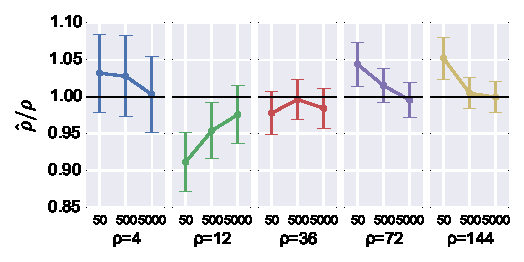
\includegraphics[width=\columnwidth]{./fig/parametric_inference/param_inference.pdf}
\caption[Inference of recombination rate $\rho$ using topological information]{Inference of recombination rate $\rho$ using topological information. The recombination rate $\rho$ is estimated for five values \{4, 12, 36, 72, 144\} at three different mutation rates \{50, 500, 5000\}. Mean estimate over 500 simulations and 95\% confidence interval is shown.}
\label{fig:param_inference}
\end{figure}

As a final point of discussion, we make a comparison with existing methods of estimating the recombination rate in coalescent models.
One of the earliest methods was developed by Hudson in \cite{Hudson:1987fo} and relies on a modeling the distribution of pairwise distances in sequence data.
Our estimator, by contrast, is built on modeling the distribution of topological features measured in the data.
In Figure~\ref{fig:estimator_comparison} we show what these distributions look like for a few values of $\rho$.
The distribution of pairwise distances follows an interesting pattern as we increase the $\rho$.
At $\rho=0$, the distances follow an exponential distribution, and as $\rho$ is increased the distances begin to follow a normal distribution with an increasingly tight variance.
That is to say, as $\rho$ is increased, all pairs of sequences begin to be normally distributed around some mean value (that is determined by the mutation rate).
Estimating $\rho$ from this data requires teasing out the contribution of recombination from the contribution of coalescence.
In contrast, our topological estimator is in some sense a more pure signal of recombination.
By the fundamental theorem, there will be no $H_1$ homology when $\rho=0$.
Any signal that is generated at $H_1$ and higher is due strictly to reticulate processes.

\begin{figure}
\centering
\subbottom[]{%
	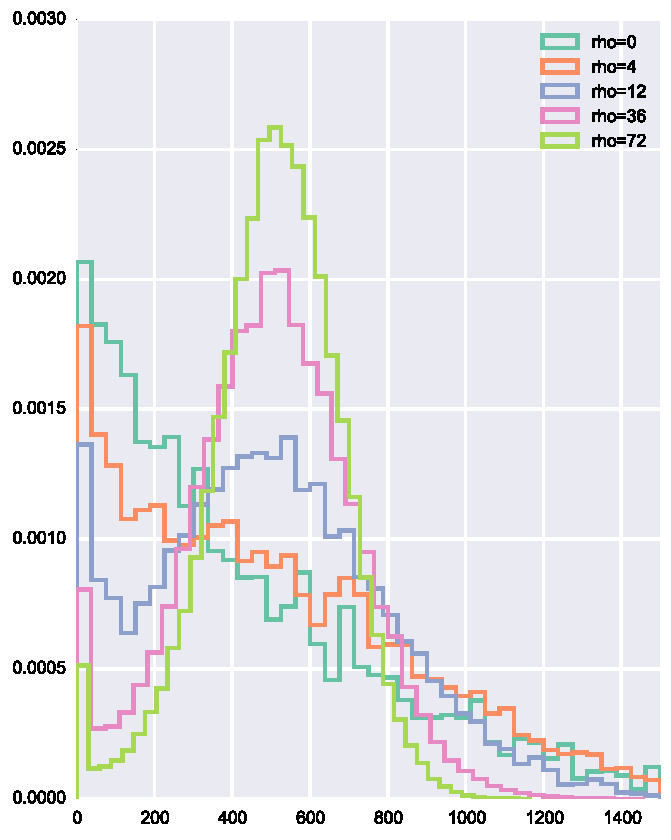
\includegraphics[width=.3\textwidth]{fig/parametric_inference/coalescent_pairwise_distance.pdf}
}
\subbottom[]{%
	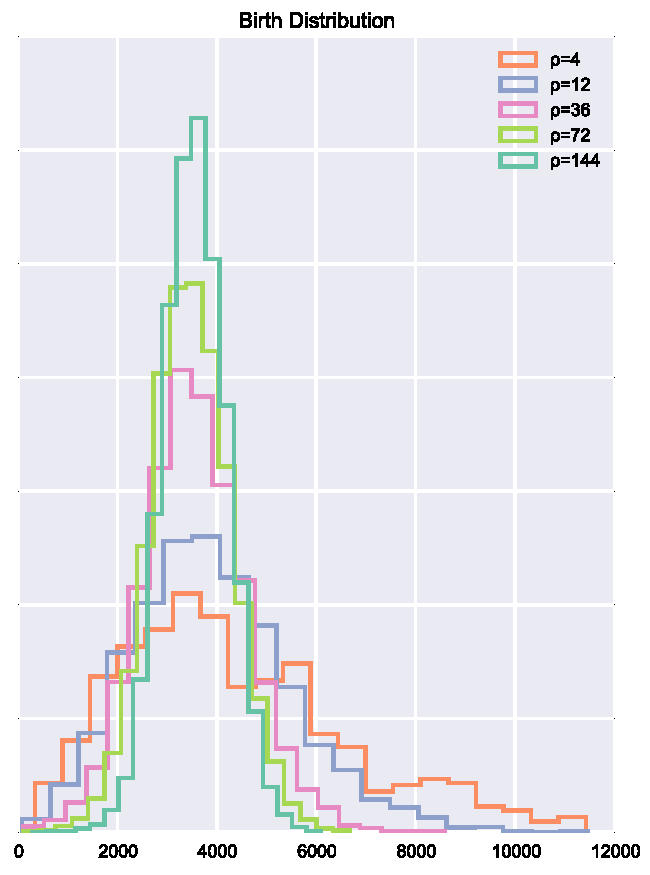
\includegraphics[width=.3\textwidth]{fig/parametric_inference/coalescent_birth_distributions.pdf}
}
\caption[Comparing traditional estimators of $\rho$ to ]{Traditional estimators of $\rho$ are based on modeling the distribution of pairwise distances in a dataset, as shown on left. This distribution is a mixture of both coalescent and recombination processes. In contrast, the distribution of birth times is driven solely by recombination.}
\label{fig:estimator_comparison}
\end{figure}

\section{Conclusions}
\label{parametric_inference:sec:discussion}

In machine learning, the task is often to infer parameters of a model from observations.
In this chapter we have presented a proof of concept for statistical inference based on topological information computed using persistent homology.
Unlike previous work, which considered estimating homology of a partially observed object, we were interested in a model which generates a complex, but stable, topological signal.
Three conditions were required for the success of this approach:
First, a well-defined statistical model.
Second, an intuition that the observed topological structure is directly correlated with the parameters of interest in the model.
Third, sufficient topological signal to reliably estimate statistics on the persistence diagram.
It is an open question to identify classes of models for which these conditions will hold.
